%%%%%%%%%%%%%%%%%%%%%%%%%%%%%%%%%%%%%%%%%%%%%%%%%%%%%%%%%%%%%%%%%%%%%%%%%%%%%%%%
% Memoria para trabajos y entregas de laboratorio de la Escuela Superior de    %
% Informática (ESI) de Ciudad Real, UCLM.                                      %
%   Versión: Octubre - 2018                                                    %
%   Desarrollada por José Ángel Martín Baos                                    %
%                                                                              %
% Recursos:			                                                           %
%   - Contenidos del curso “LaTeX esencial para preparación de Trabajo Fin de  %
%     Grado, Tesis y otros documentos académicos” impartido por el profesor    %
%     Jesús Salido.                                                            %
%                                                                              %
% Disponible en: https://github.com/JoseAngelMartinB/PlantillaTrabajosLaTeX    %
%%%%%%%%%%%%%%%%%%%%%%%%%%%%%%%%%%%%%%%%%%%%%%%%%%%%%%%%%%%%%%%%%%%%%%%%%%%%%%%%

\documentclass[11pt]{article}

% PAQUETES USADOS:
\usepackage{natbib}
\usepackage{url}
\usepackage[utf8]{inputenc} % Codificación (Permite carácteres españoles)
\usepackage{amsmath}
\usepackage{graphicx}
\graphicspath{{images/}} % Carpeta en la cual se van a buscar las imagenes
\usepackage{subfigure}	% Permite la Inclusión de subfiguras
%\usepackage{parskip} % Suprime la identación de los parrafos.
\setlength{\parskip}{3mm} % Longitud del espaciado entre parrafos
\usepackage[hidelinks]{hyperref} % Referencias (links)
\usepackage{fancyhdr}
\usepackage{vmargin}
\usepackage{paralist} % Permite un mayor control sobre las listas
\usepackage{textcomp,marvosym,pifont} % Generación de símbolos especiales
\usepackage[usenames,dvipsnames,svgnames,x11names,table]{xcolor}
\usepackage{enumerate}

% CONFIGURACIÓN DE LA PÁGINA:
\setpapersize{A4} % Formato del papel - A4
\setmarginsrb{3 cm}{2.5 cm}{3 cm}{2.5 cm}{1 cm}{1.5 cm}{1 cm}{1.5 cm} % Margenes

% Complemento para insertar código en la memoria:
%   Basado en 'Listados de código cómodos y resultones con listings'
%   de David Villa en http://crysol.org/es/node/909
\usepackage{color}
\definecolor{gray97}{gray}{.97}
\definecolor{gray75}{gray}{.75}
\definecolor{gray45}{gray}{.45}
\usepackage{listings}
\lstset{ frame=Ltb,
	framerule=0pt,
	aboveskip=0.5cm,
	framextopmargin=3pt,
	framexbottommargin=3pt,
	framexleftmargin=0.4cm,
	framesep=0pt,
	rulesep=.4pt,
	backgroundcolor=\color{gray97},
	rulesepcolor=\color{black},
	texcl=true,
	%
	stringstyle=\ttfamily,
	showstringspaces = false,
	basicstyle=\small\ttfamily,
	commentstyle=\color{gray45},
	keywordstyle=\bfseries,
	%
	numbers=left,
	numbersep=15pt,
	numberstyle=\tiny,
	numberfirstline = false,
	breaklines=true,
}
% Minimizar fragmentado de listados
\lstnewenvironment{listing}[1][]
{\lstset{#1}\pagebreak[0]}{\pagebreak[0]}

\lstdefinestyle{consola}
{basicstyle=\scriptsize\bf\ttfamily,
	backgroundcolor=\color{gray75},
}

\lstdefinestyle{C}
{language=C,
}

%OTROS PAQUETES:
\usepackage{float} % Permite usar H en las figuras, de manera que se coloquen en la posición exacta en la que están en el código.

% Añade un comando para crear indicaciones de pulsación de teclas
\usepackage{tikz} % Paquete especializado en gráficos
\usetikzlibrary{shadows} % Necesario para poder crear nuevo comando de indicación de pulsación de tecla.
\newcommand*\tecla[1]{%
	\tikz[baseline=(key.base)]
	\node[%
	draw,
	fill=white,
	drop shadow={shadow xshift=0.25ex,shadow yshift=-0.25ex,fill=black,opacity=0.75},
	rectangle,
	rounded corners=2pt,
	inner sep=1pt,
	line width=0.5pt,
	font=\scriptsize\sffamily
	](key) {#1\strut}
	;
}

\newif\ifspanish % Condicional que permite seleccionar el lenguage.
\newif\ifmultipleauthors % Condicional que permite multiples autores
\spanishtrue
\multipleauthorsfalse


%%%%%%%%%%%%%%%%%%%%%%%%%%%%%%%%%%%%%%%%%%%%%%%%%%%%%%%%%%%%%%%%%%%%%%%%%%%%%%%%
%%%%%%%%%				Principales variables del documento			   %%%%%%%%%

\title{Práctica 1: Red Hipercubo}							% Titulo
\author{David Camuñas Sánchez}							% Autor

\date{\today}											% Fecha
\newcommand{\subject}{Diseño de Infraestructuras de Red}						% Asignatura
\newcommand{\course}{Grado en Ingeniería Informática}	% Curso
%\newcommand{\course}{Máster Universitario en Ingeniería Informática}	% Curso
\newcommand{\courseyear}{2019 - 2020} 					% Curso académico
%\spanishfalse	    	% Descomentar esta línea si el trabajo está en inglés
%\multipleauthorstrue   % Descomentar esta línea si hay varios autores

%%%%%%%%%%%%%%%%%%%%%%%%%%%%%%%%%%%%%%%%%%%%%%%%%%%%%%%%%%%%%%%%%%%%%%%%%%%%%%%%

\ifspanish
	\usepackage[spanish]{babel} % Paquete de español
	\newcommand{\dateText}{Fecha:}
	\renewcommand{\lstlistingname}{Listado} % Renombrar listados para que aparezcan en español.
	% Algoritmos
	\usepackage[ruled,vlined,spanish]{algorithm2e} % Permite pseudocódigos. NECESARIO INSTALAR texlive-science (sudo apt-get install texlive-science)
\else
	\usepackage[english]{babel} % Paquete de inglés
	\newcommand{\dateText}{Date:}
	% Algoritmos
	\usepackage[ruled,vlined,english]{algorithm2e}
\fi

\makeatletter
\let\thetitle\@title
\let\theauthor\@author
\let\thedate\@date
\makeatother

% Formato de página:
\pagestyle{fancy}		% Formato por defecto - Recomendado
%\pagestyle{headings} 	% Formato para libros
\fancyhf{}
\ifmultipleauthors
	\chead{\thetitle}
\else
	\rhead{\theauthor}
	\lhead{\thetitle}
\fi
\cfoot{\thepage}

\begin{document}

%%%%%%%%%%%%%%%%%%%%%%%%%%%%%%%%%%%%%%%%%%%%%%%%%%%%%%%%%%%%%%%%%%%%%%%%%%%%%%%%
%%%%%%%%							Portada							   %%%%%%%%%

\begin{titlepage}
	\centering
	\begin{minipage}[t]{\textwidth}
		\raisebox{-0.5\height}{
\includegraphics[scale = 0.5]{uclm.jpg}} 	% Logo de la universidad
		\hspace{\fill}
		\raisebox{-0.5\height}{
\includegraphics[scale = 0.5]{open-mpi.png}} 	% Logo de open-mpi
	\end{minipage}
	\\[2.25 cm]
    \textsc{\LARGE Universidad de Castilla-La Mancha}\\[1 cm]	% Nombre de la universidad
    \textsc{\LARGE Escuela Superior de Informática}\\[2.0 cm]
	\textsc{\Large \subject}\\[0.5 cm]				% Asignatura
	\textsc{\large \course \\ \courseyear}\\[2 cm]				% Curso
	\rule{\linewidth}{0.2 mm} \\[0.4 cm]
	{ \huge \bfseries \thetitle}\\
	\rule{\linewidth}{0.2 mm} \\[2.5 cm]

	\vspace*{\fill}
	\begin{minipage}{0.4\textwidth}
		\begin{flushleft} \large
			\ifspanish
				\ifmultipleauthors
					\emph{Autores:}\\
				\else
					\emph{Autor:}\\
				\fi
			\else
				\ifmultipleauthors
					\emph{Authors:}\\
				\else
					\emph{Author:}\\
				\fi
			\fi
			\theauthor
			\end{flushleft}
			\end{minipage}~
			\begin{minipage}{0.4\textwidth}
			\begin{flushright} \large
			\emph{\dateText} \\
			\thedate
		\end{flushright}
	\end{minipage}\\[2.25 cm]


\end{titlepage}

%%%%%%%%%%%%%%%%%%%%%%%%%%%%%%%%%%%%%%%%%%%%%%%%%%%%%%%%%%%%%%%%%%%%%%%%%%%%%%%%
%%%%%%%%%						   	Índice					      	   %%%%%%%%%

\tableofcontents
\pagebreak


%%%%%%%%%%%%%%%%%%%%%%%%%%%%%%%%%%%%%%%%%%%%%%%%%%%%%%%%%%%%%%%%%%%%%%%%%%%%%%%%
%%%%%%%%%							Documento						   %%%%%%%%%
\section{Enunciado}
Dado un archivo con nombre datos.dat, cuyo contenido es una lista de valores
separados por comas, nuestro programa realizará lo siguiente:
El proceso de rank 0 destribuirá a cada uno de los nodos de un Hipercubo de
dimensión D (\textbf{$2^{D}$}), los numeros reales que estarán contenidos en el archivo
datos.dat. En caso de que no se hayan lanzado suficientes elementos de proceso
para los datos del programa, éste emitirá un error y todos los procesos
finalizarán.
En caso de que todos los procesos han recibido su correspondiente elemento,
comenzará el proceso normal del programa.
Se pide calcular el elemento mayor de toda la red, el elemento de proceso con
\textit{rank 0} mostrará en su salida estándar el valor obtenido. La complejidad del
algoritmo no superará O($log_2 (n)$).

Con n número de elementos de la red.


% Sección: Intruducción
\section{Introducción}
El objetivo de esta práctica es la creación de uno de los tipos de redes de comunicación existente, esta es la \textbf{\textit{Red Hipercubo}}.
 
Cuya peculiaridad es que son redes cuadradas, donde cada nodo o \textit{rank}, tiene \textbf{D} vecinos (uno por cada dimensión).

\begin{itemize}
	\item \textbf{Por ejemplo:} \textit{Un hipercubo de $2^3$}
	En este caso, el tamño del hipercubo es \textit{8}, esto significa, que está compuesto por 8 \textit{nodos o ranks}.
	Donde cada \textit{rank} tiene 3 \textit{vecinos}, uno por cada dimensión (D = 1, D = 2, D = 3).
\end{itemize} 

A continuación, se mostrará un ejemplo donde se puede observar varios tipos de dimensiones en un hipercubo.

\begin{figure}[H]
  \centering
    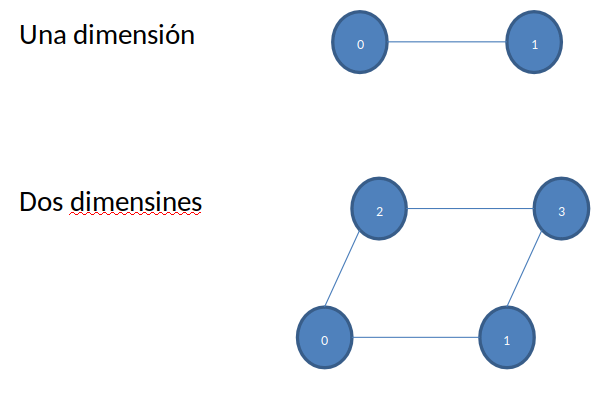
\includegraphics[width=70mm]{dimensiones.png}
  \caption{Ejemplo dimensiones de un hipercubo}
  \label{fig:matriz}
\end{figure}

\clearpage


\section{Planteamiento de la solución}
Para solucionar el problema, se tiene en cuenta que una \textit{Red Hipercubo} tiene un tamaño de $2^D$.
Donde el \textit{el valor de \textbf{D}} esta determinado por: $log_2 (D)$

En este caso el valor de \textbf{D} es \textbf{3}, por lo tanto, el tamaño \textit{(size)} será \textbf{8}, esto quiere decir que este hipercubo estaŕa formado por \textit{16 procesos} (denominados en el código como \textit{ranks}).

El número de dimensiones \textbf{D} del hipercubo se encuentra definido en \textit{la función main()}, como una constante:

\textit{\textbf{const int D = log2(size)}}

Si se quiere realizar la simulación con un valor de lado distinto, se deberá cambiar el valor del número total de procesos a crear, pasado como argumento al comando de ejecución (\textit{mpirun}) en la línea de ordenes. Este valor se puede encontrar en el \textit{Makefile} del proyecto.

Otra constante importante, es la que determina el tamaño del buffer lectura del fichero (en este caso \textit{datos.dat}), debido a que si se quiere leer una gran cantidad de números, y asi crear una gran cantidad de nodos (ranks), se debe de modificar su valor a uno mayor.

\textit{\textbf{define MAX-SIZE 1024}}

\subsection{Tipos de nodos}
En este problema encontramos dos tipos de nodos: el \textbf{\textit{rank o nodo 0}} y los demás \textbf{\textit{nodos}}.

\begin{itemize}
	\item \textbf{Rank 0}: Este nodo corresponde al primer proceso creado. Encargado de la lectura del fichero \textit{\textbf{datos.dat}}, el cual contiene los números que más tarde asignara el mismo a los demás nodos que forman la red hipercubo.
	
	A la hora de realizar la asignación de los números a los respectivos nodos restantes (incluyendose el mismo), debe de comprobar que la cantidad de números obtenidos del fichero es igual al tamaño del hipercubo \textbf{size} (nº de nodos que lo forman) si esta comprobación es exitosa, continuara la ejecución normal del programa.
	
	En caso contrario, a mi elección bien sea por que el tamaño del hipercubo o la cantidad de los números sea menor o mayor. El \textit{rank 0} cero abortará la ejecución del programa. 
	Tanto si la comprobación es correcta como si no, este difundirá el resultado a los demás nodos. Para ello se ha utilizado la función \textit{Bcast()} de la libreria de \textbf{MPI}.
	
	Una vez asignados los respectivos números a cada nodo, tras calcular el número máximo de la red hipercubo, \textit{rank 0} mostrara dicho número por pantalla, y el programa finalizará.
	
	\item \textbf{Los demás nodos}: Estos tipos de nodos recibirán del \textit{rank 0} la decisión de continuar o no. Si continua la ejecución normal se les asignará un número real, el cual trás obtener cada uno sus respectivos vecinos, se  llevará a cabo el algoritmo para obtener \textit{el menor número de la red hipercubo}.
\end{itemize}


\subsection{Algoritmos principales}
Los algoritmos principales de esta práctica son: \textbf{la obtención de los vecinos} (de cada nodo) y \textbf{cálculo del número máximo} de la red hipercubo.

\subsubsection{Obtención de los vecinos}
Este algoritmo es fundamental en el programa, debido a que gracias a el se ve de una manera más intutiva la estructura de la red hipercubo, donde cada nodo o rank conoce a sus respectivos vecinos. Cada nodo tiene un total de \textit{D vecinos}, almacenador en el vector de tipo entero denominado \textit{neighbors} (vecinos).

En este caso, los vecinos de se han obtenido mediante el cambio de los bits que forman el \textit{rank} del nodo actual, en este caso según el rank que sea se han cambiado los bits dependiendo de la dimensión a la que pertenezca el vecino.

Este proceso se ha realizado con la ayuda de la operación lógica \textit{XOR}, entre el \textit{rank} actual más la dirección generada por cada dimensión.
En la sección corresondiente al algoritmo se explicara de forma más páctica el proceso que sigue.

\begin{figure}[H]
  \centering
    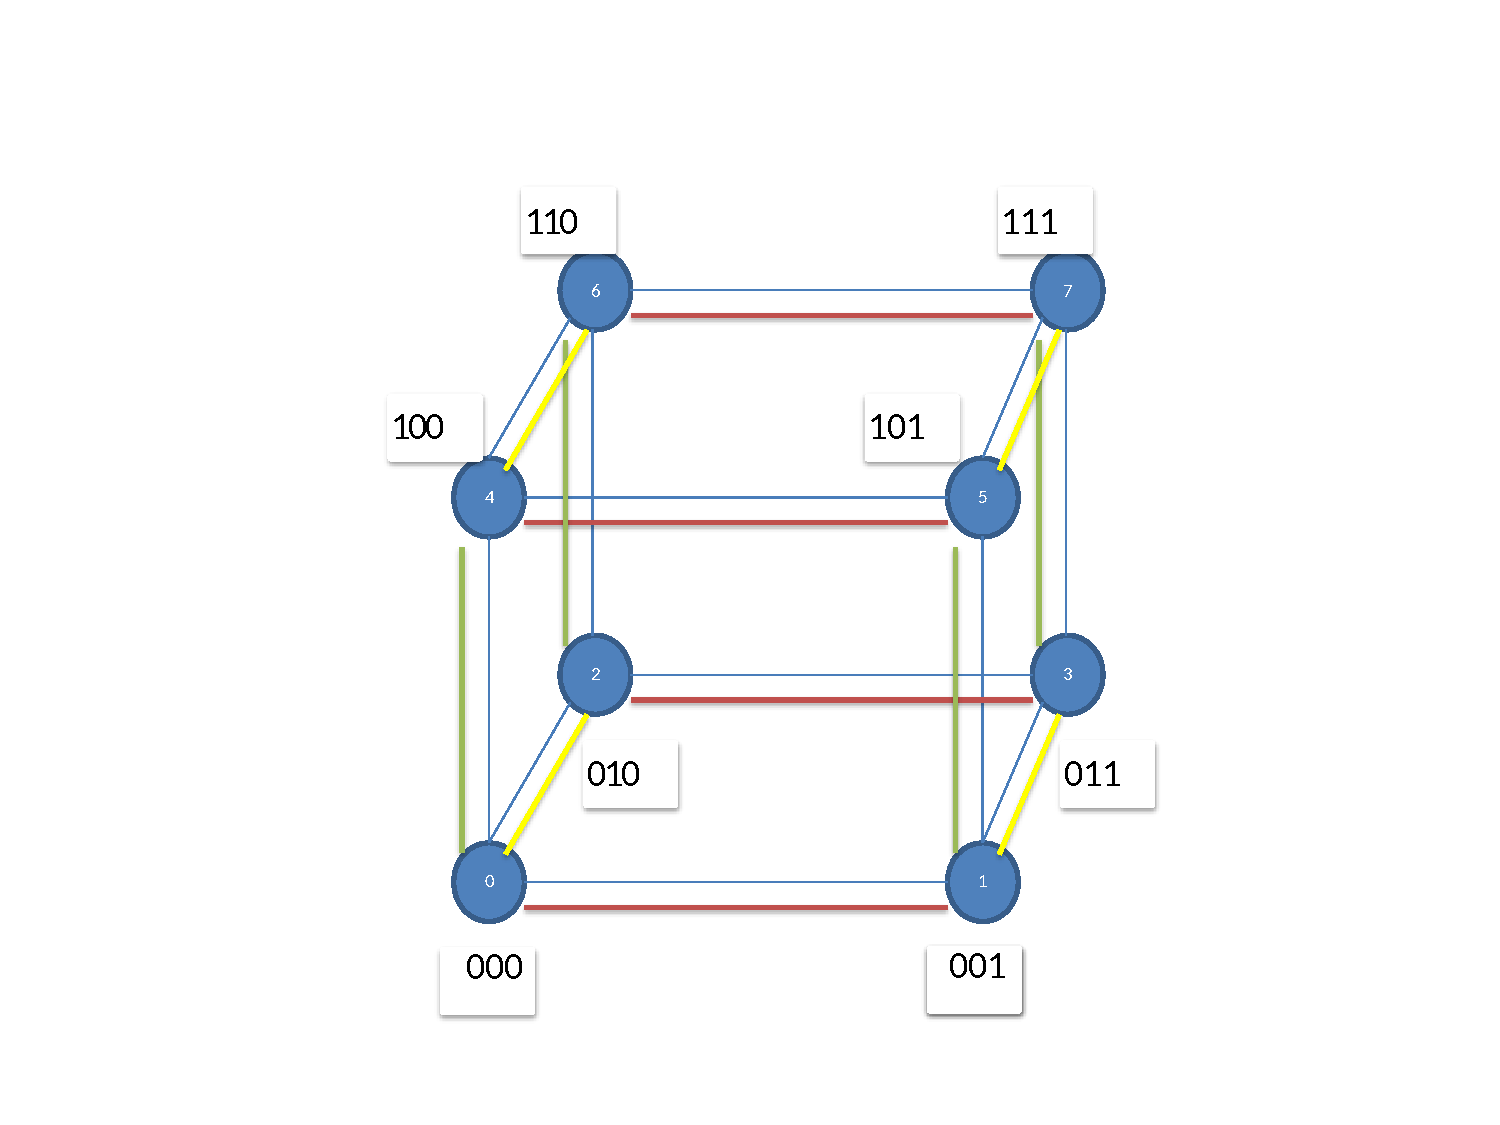
\includegraphics[width=95mm]{hipercubo.pdf}
  \caption{Representación red hipercubo $2^3$ con los respectivos ranks.}
  \label{fig:matriz}
\end{figure}


\subsubsection{Cálculo del número máximo}
El segundo algoritmo principal de este programa, es el de cálcular el número máximo de toda la red hipercubo, para ello cada nodo ira comprobando su número y el de sus vecinos y se quedara con el mayor de ellos, esta comnprobación la realizará enviando su numero a cada vecino y recogiendo el de cada vecino para comprobarlo con el suyo.

Al realizar este proceso cada nodo, a nivel global se realizará para todos los nodos de la red, entonces de esta forma al tener cada nodo vecinos que a la vez ellos mismos son vecinos de otros nodos, todos los nodos se quedarán finalmente con el número mayor de toda la red hipercubo.

La secuencia de acciones de este algoritmo es la siguiente:
\begin{enumerate}
	\item Intercambio de números entre vecino de cada dimensión.
	\item Comparación entre el número actual y el recibido, quedandose el nodo actual con el número máximo.

\begin{figure}[H]
  \centering
  \subfigure{
    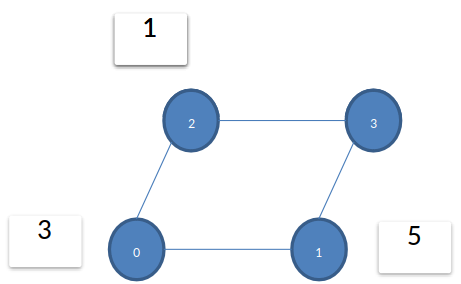
\includegraphics[width=36mm]{inicio.png}
  }
  \subfigure{
  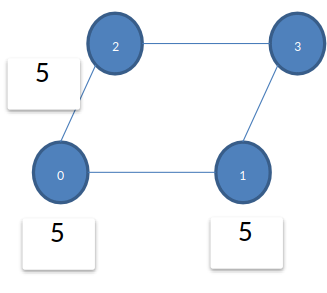
\includegraphics[width=22mm]{fin.png}
  }
  \caption{Reprersentación cálculo del valor máximo de un rank y sus vecinos}
  \label{fig:toroide}
\end{figure}
\end{enumerate}

\clearpage

\section{Diseño de la solución}
A continuación, se explicarán las funciones que forman parte del programa, el cual da una solución al enunciado de esta práctica.
\\

\subsection{Función principal del programa (\textit{main})}
Esta es la función principal del programa, en la cual como se puede observar lo primero que se lleva a cabo es la definicion de las variables a utilizar, como: \textit{rank}, \textit{numbers-n} (cantidad de números), \textit{size} (tamaño del hipercubo), \textit{data} (vector donde se almacenarán los números obtenidos del fichero), etc.

Tras esto se declarán las primitivas de \textit{\textbf{MPI}} como: 
\begin{itemize}
	\item textit{MPI-Init}() para inicializar la estructura de comunicación de MPI entre los procesos. 
	\item \textit{MPI-Comm-Size}() para obtener el tamaño de la comunicacion (número de proceso a ejecutar en este caso, ranks), etc.
	\item \textit{MPI-Comm-rank() Para establecer el identificador de cada proceso \textit{rank}}.
\end{itemize}

También esta función se lleva a cabo las llamadas a las demás tipos de funciones que componen el programa

\lstinputlisting[language=C]{code/main.c}

\subsection{Lectura del fichero (\textit{load-data})}
La primera función a llamar dentro del \textit{main}, es la \textit{load-data()}, encargada de la lectura del fichero, esta función añade los números que almacena el fichero al vector de tipo \textit{long double} denominado \textit{data}.
Esta función obitiene los números del fichero, seprarando cada uno utilizando como separador la \textit{coma}.\\

Para la apertura del fichero se ha utilizado la función \textit{open-file()}, cuyo principal objetivo es devolver el descriptor del archivo \textit{datos.dat}.
A esta función se le pasa como parámetro \textit{DATA-PATH} que es la ruta del archivo a leer y \textit{READ-MOD} que indica el modo de apertura del archivo, en este caso el modo de lectura.
\lstinputlisting[language=C]{code/open_file.c}

Una vez cargados los datos en el vector \textit{data}, la función devolverá la variable \textit{i}, la cual almacena el valor de la cantidad de números que contiene el fichero.
\lstinputlisting[language=C]{code/load_data.c}

\subsection{Comprobación de la cantidad de números (\textit{check-size})}
Esta función se encarga de comprobar si la cantidad de números (\textit{numbers-n}) es igual al tamaño (\textit{size}) del hipercubo. Estos son los argumentos que se les pasa a la función.
La función devolverá True o False si es igual o no estas variables, si la devolución es False, entonces finalizará la ejecución normal del programa. Y el proceso \textit{rank 0}, mandará una difusión a los demás procesos, para que asi aborten su ejecución. Esto se realiza con la primitiva \textit{MPI-Bcast()}. 

\lstinputlisting[language=C]{code/bdcast.c}

\lstinputlisting[language=C]{code/check_size.c}


\subsection{Envio de su número a cada nodo (\textit{add-numbers})}
Esta función tiene el objetivo de añadir o enviar a cada nodo (\textit{rank}) su número, esta tarea es realizada por\textit{rank 0}.

Tanto para el envio como para la recepción del nodo se han utilizado las primitivas basicas de MPI (\textit{MPI-Send y MPI-Recv}).
Esta función recoge como parámetros el vector \textit{data} y la variable entera \textit{size} (tamaño hipercubo).

\lstinputlisting[language=C]{code/add_numbers.c}

Por último, se libera el espacio de memoria reservado para el vector de números \textit{data}.


\subsection{Obtención de los vecinos (\textit{get-neighbors})}
Esta función se encarga de que cada proceso, obtenga el rank de cada vecino, es decir, de sus vecinos \textit{de cada dimensión}. Para ello esta función recogerá como parámetros el rank del proceso que la ejecute, y su lista de vecinos vacía en este caso, representada mediante el vector de enteros llamado \textit{neighbors} (pasada por referencia).

Esta función es muy importante para la función que cálcula el máximo número de la red hipercubo \textit{calculate-max()}, debido que aquí cada nodo o rank conoce quienes son sus vecinos, con los cuales realizará dicha comprobación intercambiando sus números.

El objetivo y funcionamiento de este algoritmo se ha explicado de una forma más teórica en el apartado 2, en concreto, la sección 2.2.1.

\lstinputlisting[language=C]{code/get_neighbors.c}

Como se puede observar el proceso de obtención se debide en dos partes, generación de la dirección de 4 bits dependiendo de la dimensión, y la \textit{XOR} entre el \textit{rank} y el rank generado por la dimensión.

\begin{itemize}
	\item \textbf{Generación del número}: dependiendo de la dimensión en la que nos encontremos se cambiara ese bit empezando de forma creciente a partir del menos significativo, es decir, por la derecha. Esto se denomina también desplazamiento del bit, cambiando asi esa posición por un 1. Y asi obtendrfiamos el número de esa dimensión
	\item \textbf{Dirección XOR \textit{rank}}: una vez generado lo que sería el rank de dicha dimensión, se realiza una operación XOR entre el número generado y el rank actual. El resultado sera el \textit{rank del vecino} de esa dimensión del nodo actual.
\end{itemize}

Tras estas operaciones se añadira dicho rank del vecino al vector de vecinos (\textit{neighbors}).

\subsection{Cálculo del número máximo (\textit{calculate-min})}
El objetivo principal de esta función es la del cálculo del número máximo de la red hipercubo, en el cual todos los elementos de la red deben de contener finalmente el número máximo.

Para ello se explicará a continuaicón de una forma más práctica el procedimiento de este algoritmo, dado que en la sección 2.2.2 ya ha sido explicado de una forma más teoríca.

----------------

\lstinputlisting[language=C]{code/calculate-v1.c}


Un ejemplo de representación del estado de la red, en un inicio y al final, tras haber calculado el máximo, seria el siguiente:

\begin{figure}[H]
  \centering
  \subfigure{
    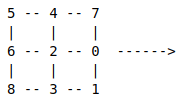
\includegraphics[width=38mm]{matriz-ini.png}
  }
  \subfigure{
  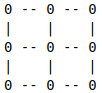
\includegraphics[width=22mm]{matriz-fin.png}
  }
  \caption{Representación red hipercubo al inicio y al final}
  \label{fig:toroide}
\end{figure}

\clearpage

 

%%%%%%%%%%%%%%%%%%%%%%%%%%%%%%%%%%%%%%%%%%%%%%%%%%%%%%%%%%%%%%%%%%%%%%%%%%%%%%%%
%%%%%%%%% 						BIBLIOGRAFIA 						   %%%%%%%%%
%%%%%%%%%%%%%%%%%%%%%%%%%%%%%%%%%%%%%%%%%%%%%%%%%%%%%%%%%%%%%%%%%%%%%%%%%%%%%%%%
\newpage
\bibliography{biblist}
\bibliographystyle{plain}
%\nocite{*} Permite citar todas las referencias en el archivo .bib

% Añadir la bibliografía al Índice de contenidos
\ifspanish
	\addcontentsline{toc}{section}{Referencias}
\else
	\addcontentsline{toc}{section}{References}
\fi




\end{document}
